\documentclass[11pt]{article}
\usepackage[italian]{babel}
\usepackage[utf8]{inputenc}	% Para caracteres en español
\usepackage{amsmath,amsthm,amsfonts,amssymb,amscd}
\usepackage{multirow,booktabs}
\usepackage[table]{xcolor}
\usepackage{fullpage}
\usepackage{lastpage}
\usepackage{enumitem}
\usepackage{fancyhdr}
\usepackage{mathrsfs}
\usepackage{wrapfig}
\usepackage{graphicx}
\graphicspath{ {./images/} }
\usepackage{setspace}
\usepackage{calc}
\usepackage{multicol}
\usepackage{cancel}
\usepackage[retainorgcmds]{IEEEtrantools}
\usepackage[margin=3cm]{geometry}
\usepackage{amsmath}
\newlength{\tabcont}
\setlength{\parindent}{0.0in}
\setlength{\parskip}{0.05in}
\usepackage{empheq}
\usepackage{framed}
\usepackage[most]{tcolorbox}
\usepackage{xcolor}
\usepackage{FiraSans}
\colorlet{shadecolor}{orange!15}
\parindent 0in
\parskip 12pt
\geometry{margin=1in, headsep=0.25in}
\theoremstyle{definition}
\newtheorem{defn}{Definizione}
\newtheorem{reg}{Regola}
\newtheorem{oss}{Osservazione}
\newtheorem{exer}{Esecizio}
\newtheorem{note}{Nota}
\newtheorem{thm}{Teorema}[section] % reset theorem numbering for each chapter
\theoremstyle{plain}
\newcommand{\restr}[2]{%
\mathchoice{%
\restriction{#1}{#2}{\displaystyle}%
}{%
\restriction{#1}{#2}{\textstyle}%
}{%
\restriction{#1}{#2}{\scriptstyle}%
}{%
\restriction{#1}{#2}{\scriptscriptstyle}%
}%
}

\newlength{\totbarheight}
\newlength{\bardepth}




\begin{document}

\title{Regressione Lineare}
\author{Guglielmo Bartelloni}
\maketitle

\thispagestyle{empty}

\begin{center}
{\LARGE \bf 30 Marzo 2022}\\
\end{center}

Possiamo avere rumore nei dati, ovvero i dati possono venire da misure sperimentali affette da errore.

\section{Approssimazione Polinomiale nel senso dei minimi quadrati}

Supponiamo di avere un campione di dati, $(x_{i},f_{i})$, per $i=0,...,N$ in cui $f_{i}=\sum_{i=0}^{m} a_kx_{i}^{k}$  con $m<<N$ 
(Abbiamo pochi dati che rispettano le condizioni di interpolazione).

(Assumiamo che almeno m+1 delle ascisse $x_{i}$ siano tra loro distinte)

Quello che dobbiamo fare e' quindi quello di calcolare i coefficienti $a_0,...,a_m$ che meglio approssimano i dati del problema.

Un criterio per questo, consiste nel chiamare $y_{i}=\sum_{k=0}^{m} a_kx_{i}^{k}$ il valore \textbf{previsto} dal modello polinomiale e, definendo i 2 vettori:
\[
	f=[f_0,f_1,...,f_N]^{T}
.\] 
\[
	Y=[y_0,y_1,....,y_N]^{T}
.\] 

Minimizzare la norma della loro differenza:
\[
||f-Y||
.\] 

Questa norma, per quello che andremo a vedere, e' scelta come norma 2. Il motivo di questo deriva dal fatto che:

Y e' una matrice con in ogni riga

Immagine appunti

\begin{oss}
	Se almeno m+1 delle ascisse ${x_{i}}$ sono distinte tra loro, le corrispondenti righe definiscono una matrice di Vandermonde non singolare.

	Pertanto, $rank(V)=m+1$, ovvero la matrice $V\in R^{N+1xm+1}$ ha \textbf{rango massimo}. 
\end{oss}

Quindi desideriamo calcolare il vettore $a$  come soluzione del sistema lineare sovradeterminato:
	\[
		Va=f\ (**)
	.\] 

Pertanto, se in (*) utilizziamo la norma 2, questo equivale a risolvere (**) nel senso dei minimi quadrati, mediante la fattorizzazione QR della matrice V. 

	I coefficienti, che sono le componenti del vettore $a$, definiscono il \textbf{polinomio di approssimazione ai minimi quadrati} dei dati $(x_{i},f_{i})$ per $i=0,...,N$ 

	\begin{oss}
		Se m=N si ottiene il polinomio interpolante, in quanto si soddisfano esattamente le condizioni:
		\[
		\sum_{k=0}^{m} a_kx_{i}^{k}=f_{i}\ \ \ i=0,...,m
		.\] 
	\end{oss}

La function \textbf{polyfit} di Matlab implementa l'approssimazione polinomiale ai minimi quadrati.

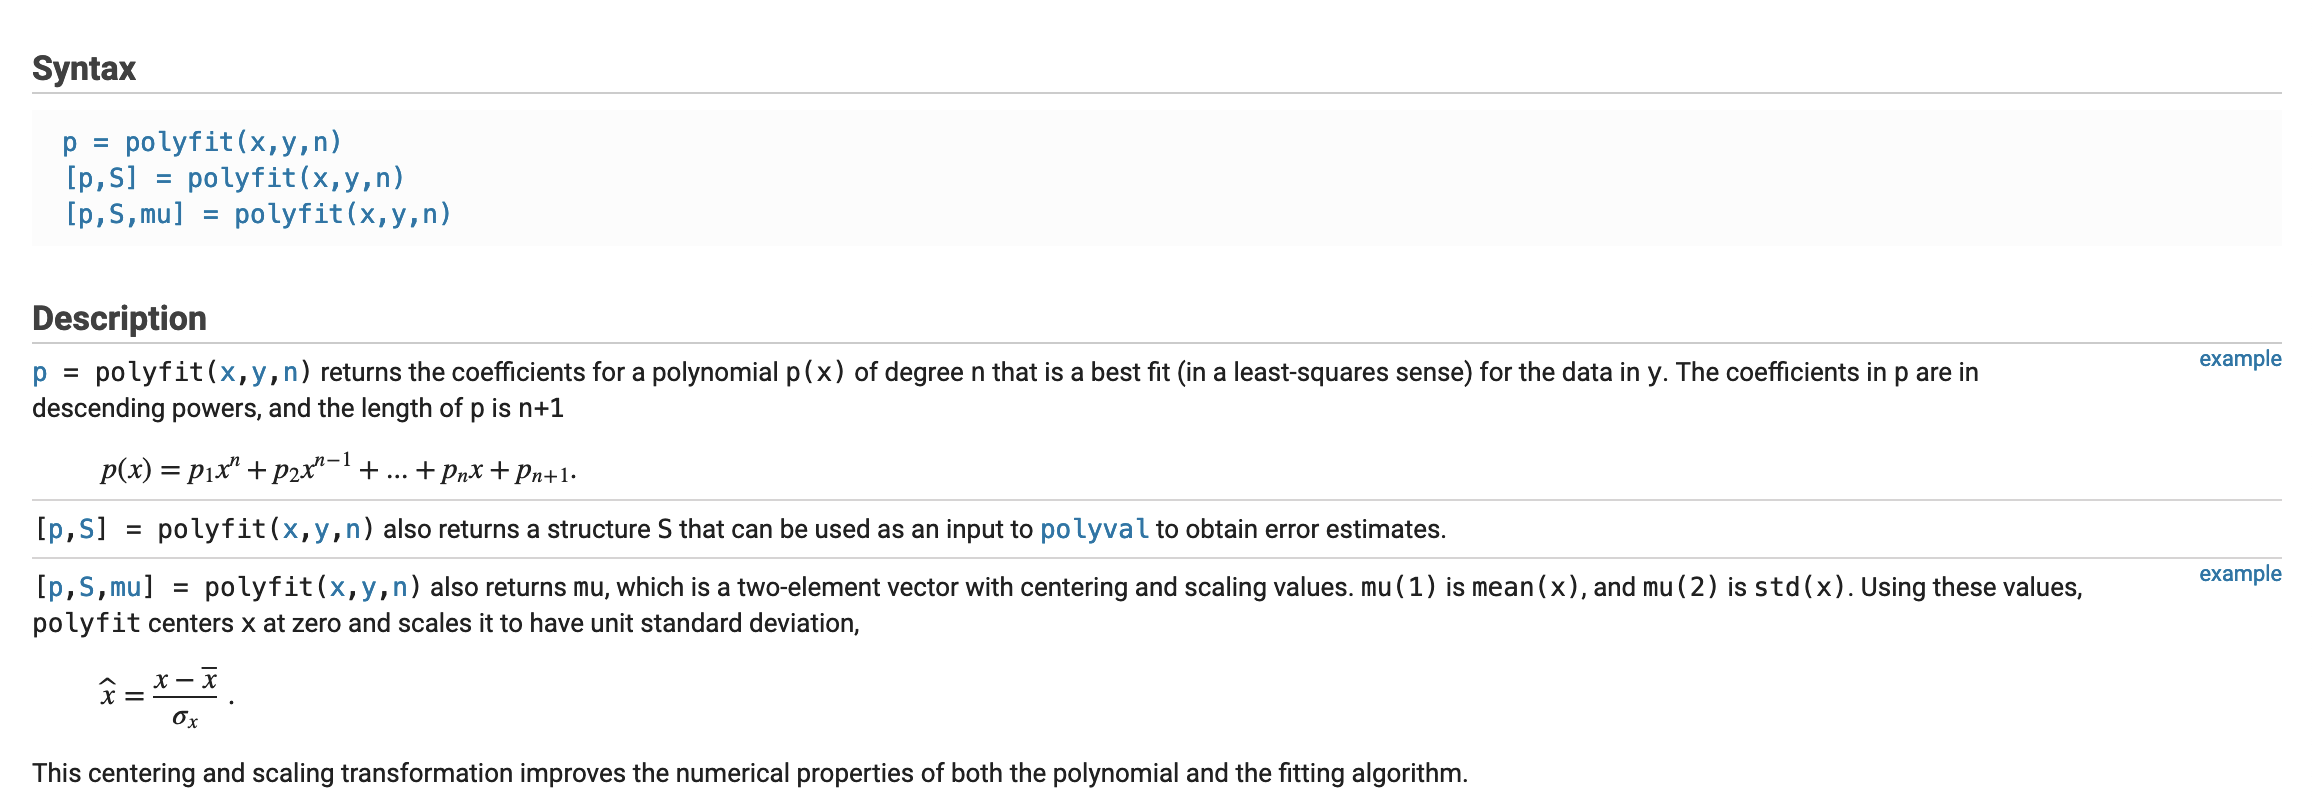
\includegraphics[width=\textwidth]{polyfit}



\end{document}
